% Two schematic zero sets in R^3.  All conclusions concern 2-dimensional currents.
% The transverse line in the left panel is not part of the current support.
\begingroup
\centering
\resizebox{\linewidth}{!}{%
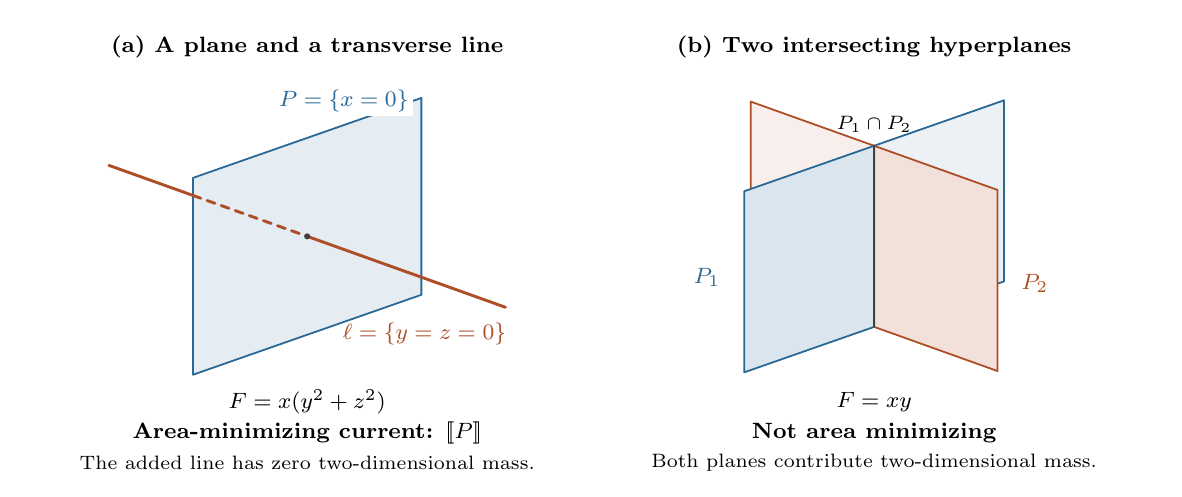
\begin{tikzpicture}[x=1cm,y=1cm,line cap=round,line join=round,
  font=\footnotesize]
  \definecolor{coneplane}{RGB}{42,104,149}
  \definecolor{coneline}{RGB}{173,78,39}
  \tikzset{plane edge/.style={draw=coneplane,line width=.65pt},
    second edge/.style={draw=coneline,line width=.65pt}}
  % The fixed bounding box makes the two panels equally wide.
  \path[use as bounding box] (-3.55,-2.95) rectangle (10.75,2.65);

  \begin{scope}
    \node[font=\footnotesize\bfseries] at (0,2.4)
      {(a) A plane and a transverse line};
    % P={x=0}; projected y- and z-directions are (1,.35) and (0,1).
    \filldraw[plane edge,fill=coneplane!12]
      (-1.45,-1.7575)--(1.45,-.7425)--(1.45,1.7575)--(-1.45,.7425)--cycle;
    % The x-axis has projected direction (.95,-.34).  Its rear segment is
    % dashed precisely where it lies behind the displayed patch of P.
    \draw[coneline,line width=1.05pt] (-2.5175,.901)--(-1.45,.51895);
    \draw[coneline,line width=1.05pt,dash pattern=on 3pt off 2.4pt]
      (-1.45,.51895)--(0,0);
    \draw[coneline,line width=1.05pt] (0,0)--(2.5175,-.901);
    \fill[black!75] (0,0) circle (1.1pt);
    \node[coneplane,anchor=south east,fill=white,inner sep=1.6pt]
      at (1.35,1.52) {$P=\{x=0\}$};
    \node[coneline,anchor=north east] at (2.65,-.98)
      {$\ell=\{y=z=0\}$};
    \node at (0,-2.1) {$F=x(y^2+z^2)$};
    \node[font=\footnotesize\bfseries] at (0,-2.5)
      {Area-minimizing current: $[\![P]\!]$};
    \node[font=\scriptsize] at (0,-2.87)
      {The added line has zero two-dimensional mass.};
  \end{scope}

  \begin{scope}[xshift=7.2cm]
    \node[font=\footnotesize\bfseries] at (0,2.4)
      {(b) Two intersecting hyperplanes};
    % P_1={x=0}, P_2={y=0}.  Draw the rear half-planes first, then the
    % front half-planes, so both sheets and their intersection are visible.
    \filldraw[plane edge,fill=coneplane!9]
      (0,-1.15)--(1.65,-.5725)--(1.65,1.7275)--(0,1.15)--cycle;
    \filldraw[second edge,fill=coneline!9]
      (-1.5675,-.589)--(0,-1.15)--(0,1.15)--(-1.5675,1.711)--cycle;
    \filldraw[plane edge,fill=coneplane!17]
      (-1.65,-1.7275)--(0,-1.15)--(0,1.15)--(-1.65,.5725)--cycle;
    \filldraw[second edge,fill=coneline!17]
      (0,-1.15)--(1.5675,-1.711)--(1.5675,.589)--(0,1.15)--cycle;
    \draw[black!75,line width=.9pt] (0,-1.15)--(0,1.15);
    \node[coneplane,anchor=east] at (-1.83,-.52) {$P_1$};
    \node[coneline,anchor=west] at (1.75,-.6) {$P_2$};
    \node[anchor=south,font=\scriptsize] at (0,1.2) {$P_1\cap P_2$};
    \node at (0,-2.1) {$F=xy$};
    \node[font=\footnotesize\bfseries] at (0,-2.5)
      {Not area minimizing};
    \node[font=\scriptsize] at (0,-2.87)
      {Both planes contribute two-dimensional mass.};
  \end{scope}
\end{tikzpicture}
}
\par
\endgroup
